\newpage
\subsection*{Task 3}

\subsubsection*{b)}

\begin{figure}[h!]
    \centering
    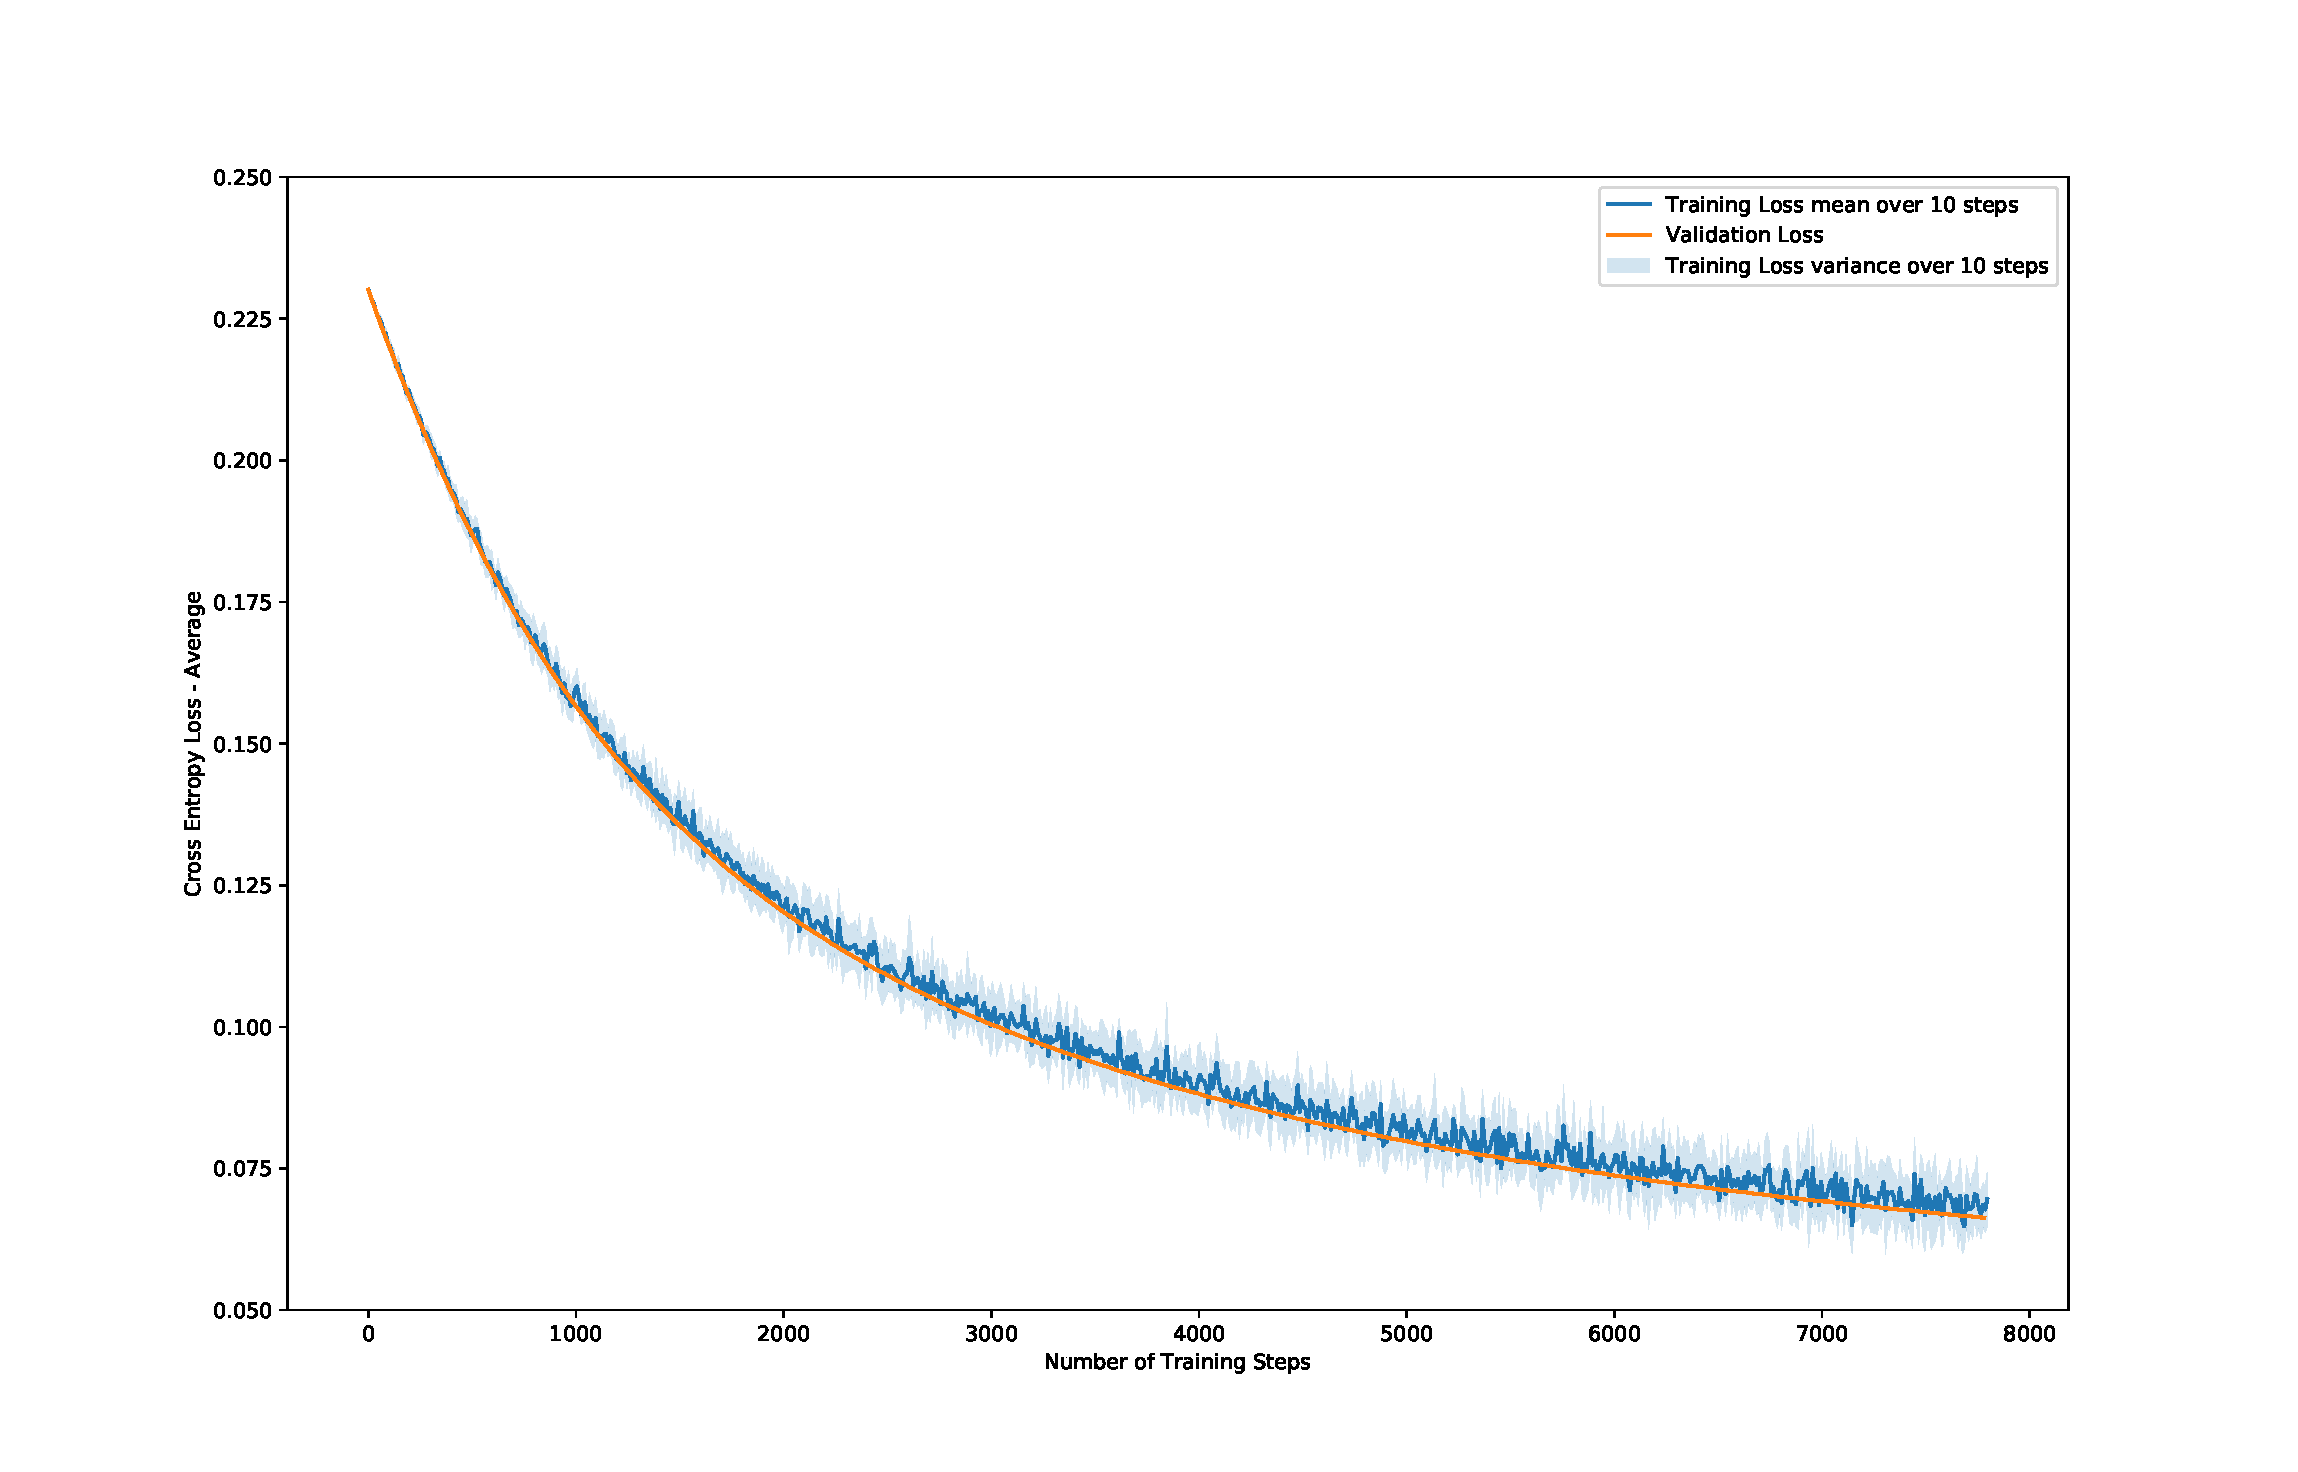
\includegraphics[clip, trim=0cm 0cm 0cm 0cm,width=0.85\textwidth]{figures/Task3b.pdf}
    \caption{Training and validation loss over training.}
    \label{fig:task3:train_val_loss}
\end{figure}

\subsubsection*{c)}

\begin{figure}[h!]
    \centering
    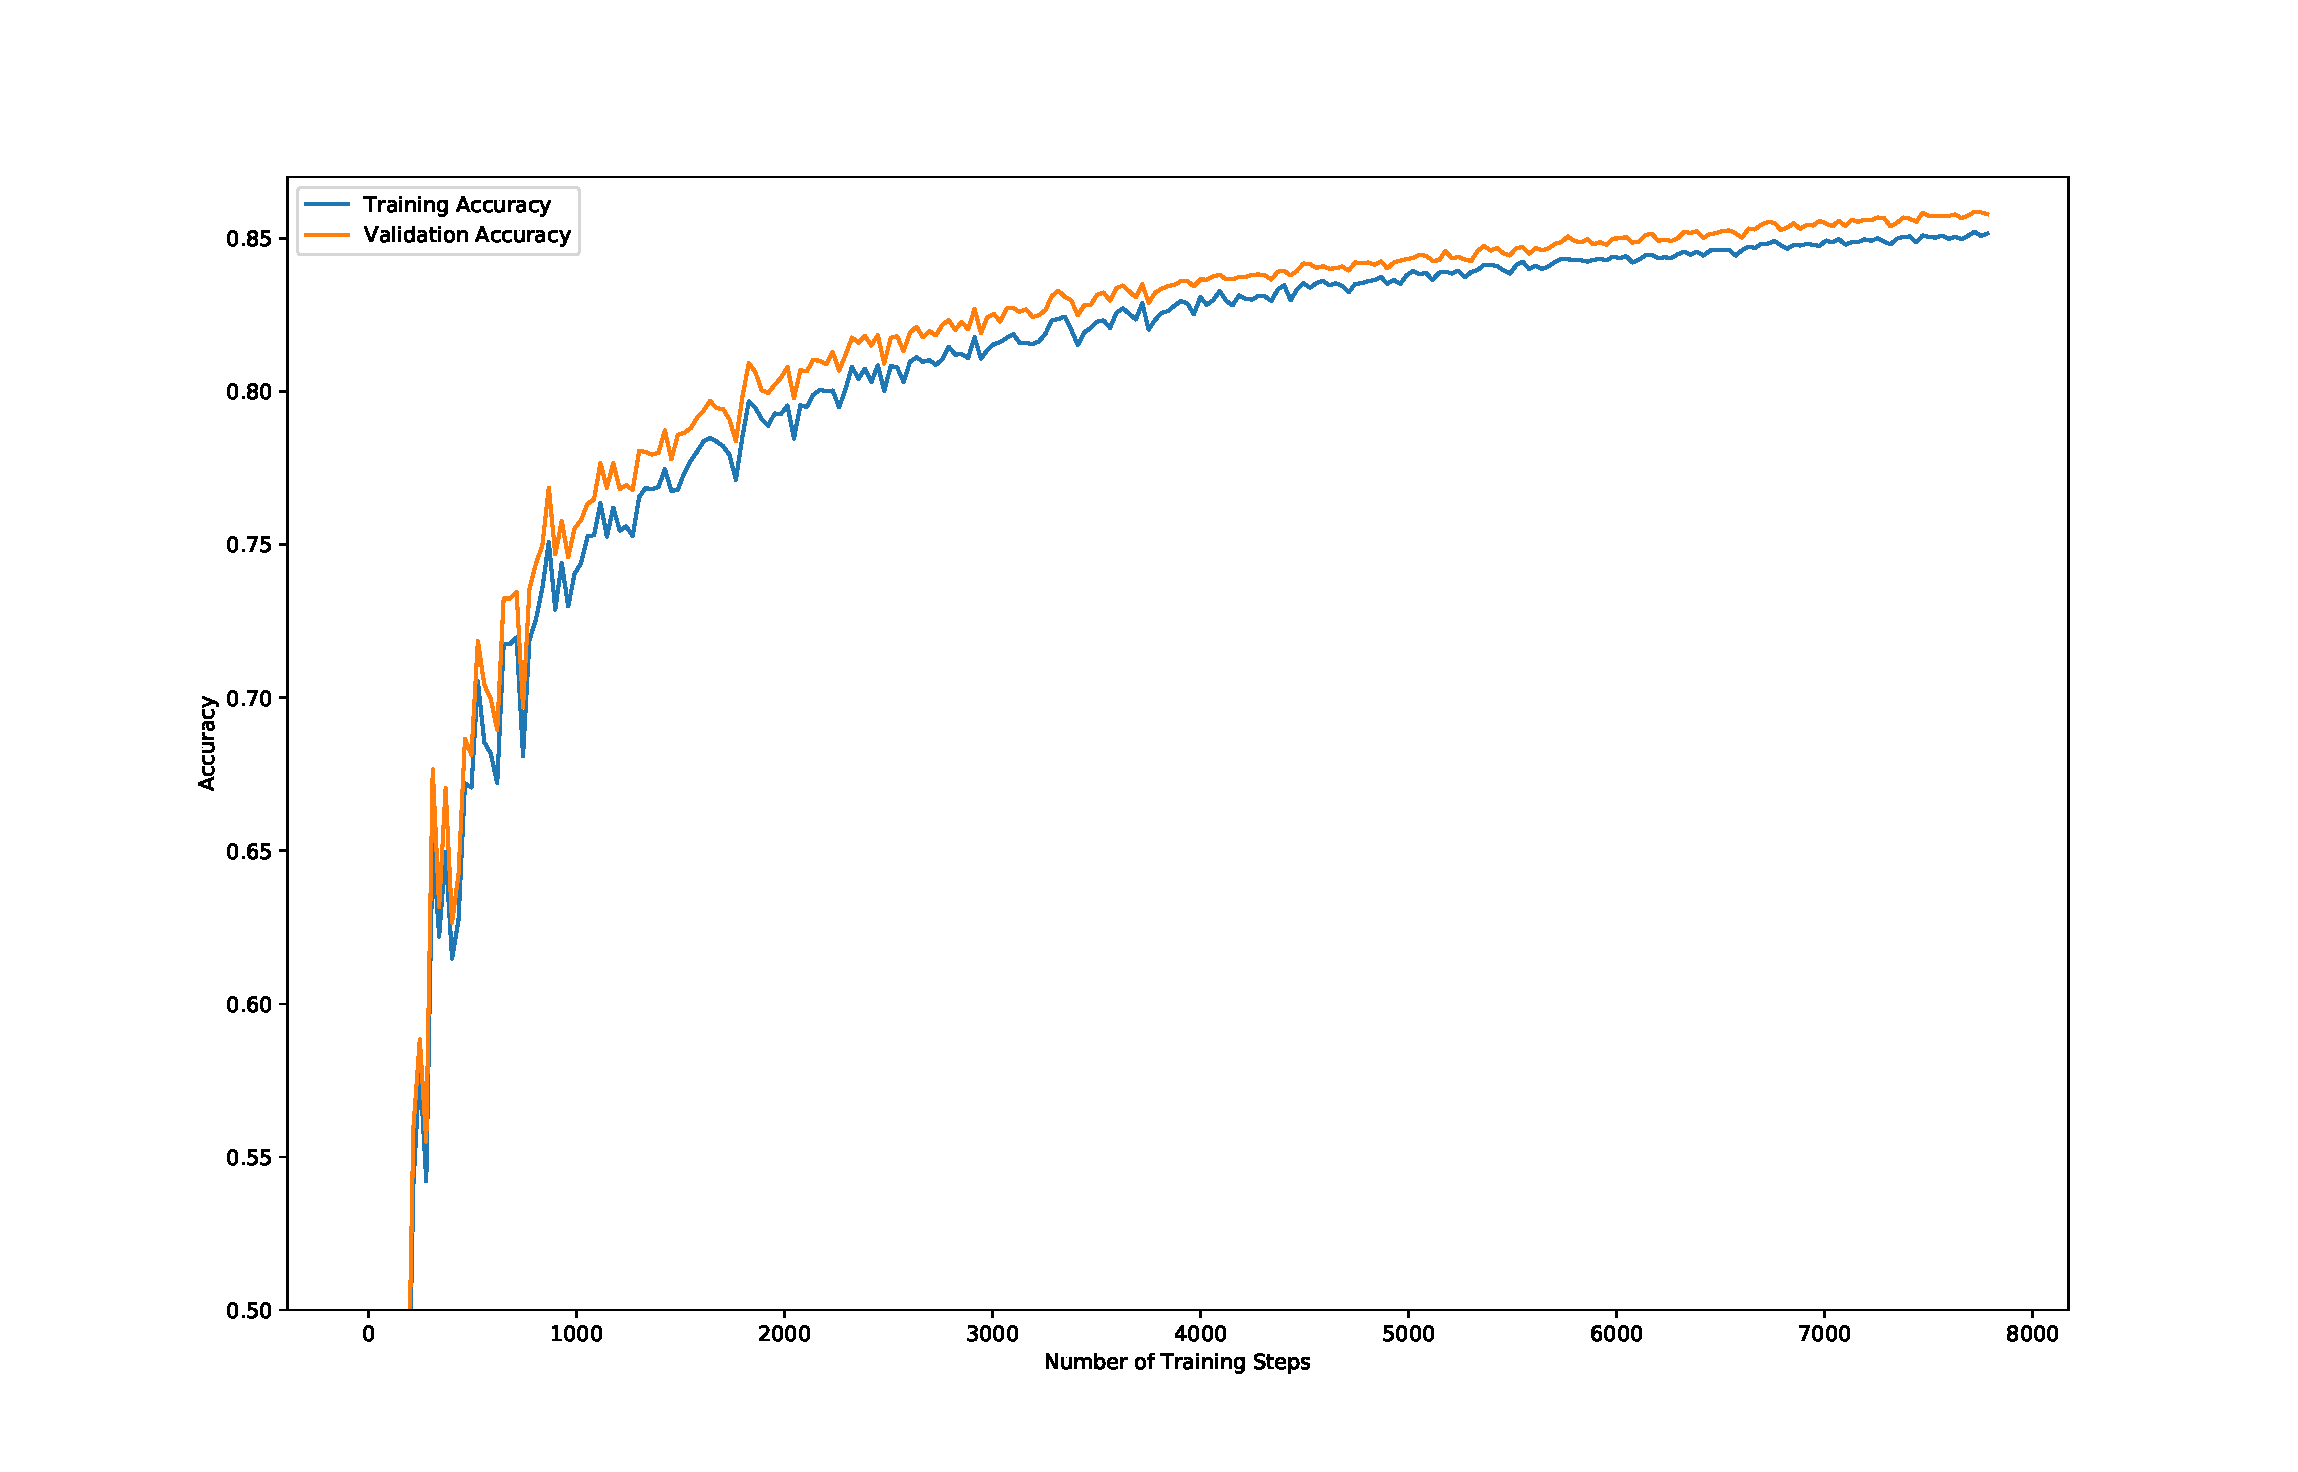
\includegraphics[clip, trim=0cm 0cm 0cm 0cm,width=0.85\textwidth]{figures/Task3c.pdf}
    \caption{Accuracy on training and validation set over training.}
    \label{fig:task3:accuracy}
\end{figure}

\subsubsection*{d)}
From \cref{fig:task3:train_val_loss} and \cref{fig:task3:accuracy} we see that the validation set loss and accuracy follows the training set, so we cannot say there are signs of overfitting based on this. One would typically see that the validation set accuracy deterioates after a while when overfitting, and that the training set achieves a lower loss and greater accuracy than the validation set. As this is not the case, we cannot say there are signs of overfitting, but a test set would help determining this. We should however not exclude overfitting solely based on the validation set, as the data in the validation set may be very similar to the training set, and therefore not represent the whole distribution of data well enough. However, I think it is odd that the model acheives better accuracy on the validation set than on the training set, so there may be something wrong in the code.
